\documentclass{standalone}
\usepackage{tikz}
\usetikzlibrary{calc}
\newcommand\N{9}
\newcommand\NM{8}	%N-1
\newcommand\NMM{7}	%N-2
\newcommand\m{4}
\newcommand\bm{9}	%2m+1
\begin{document}
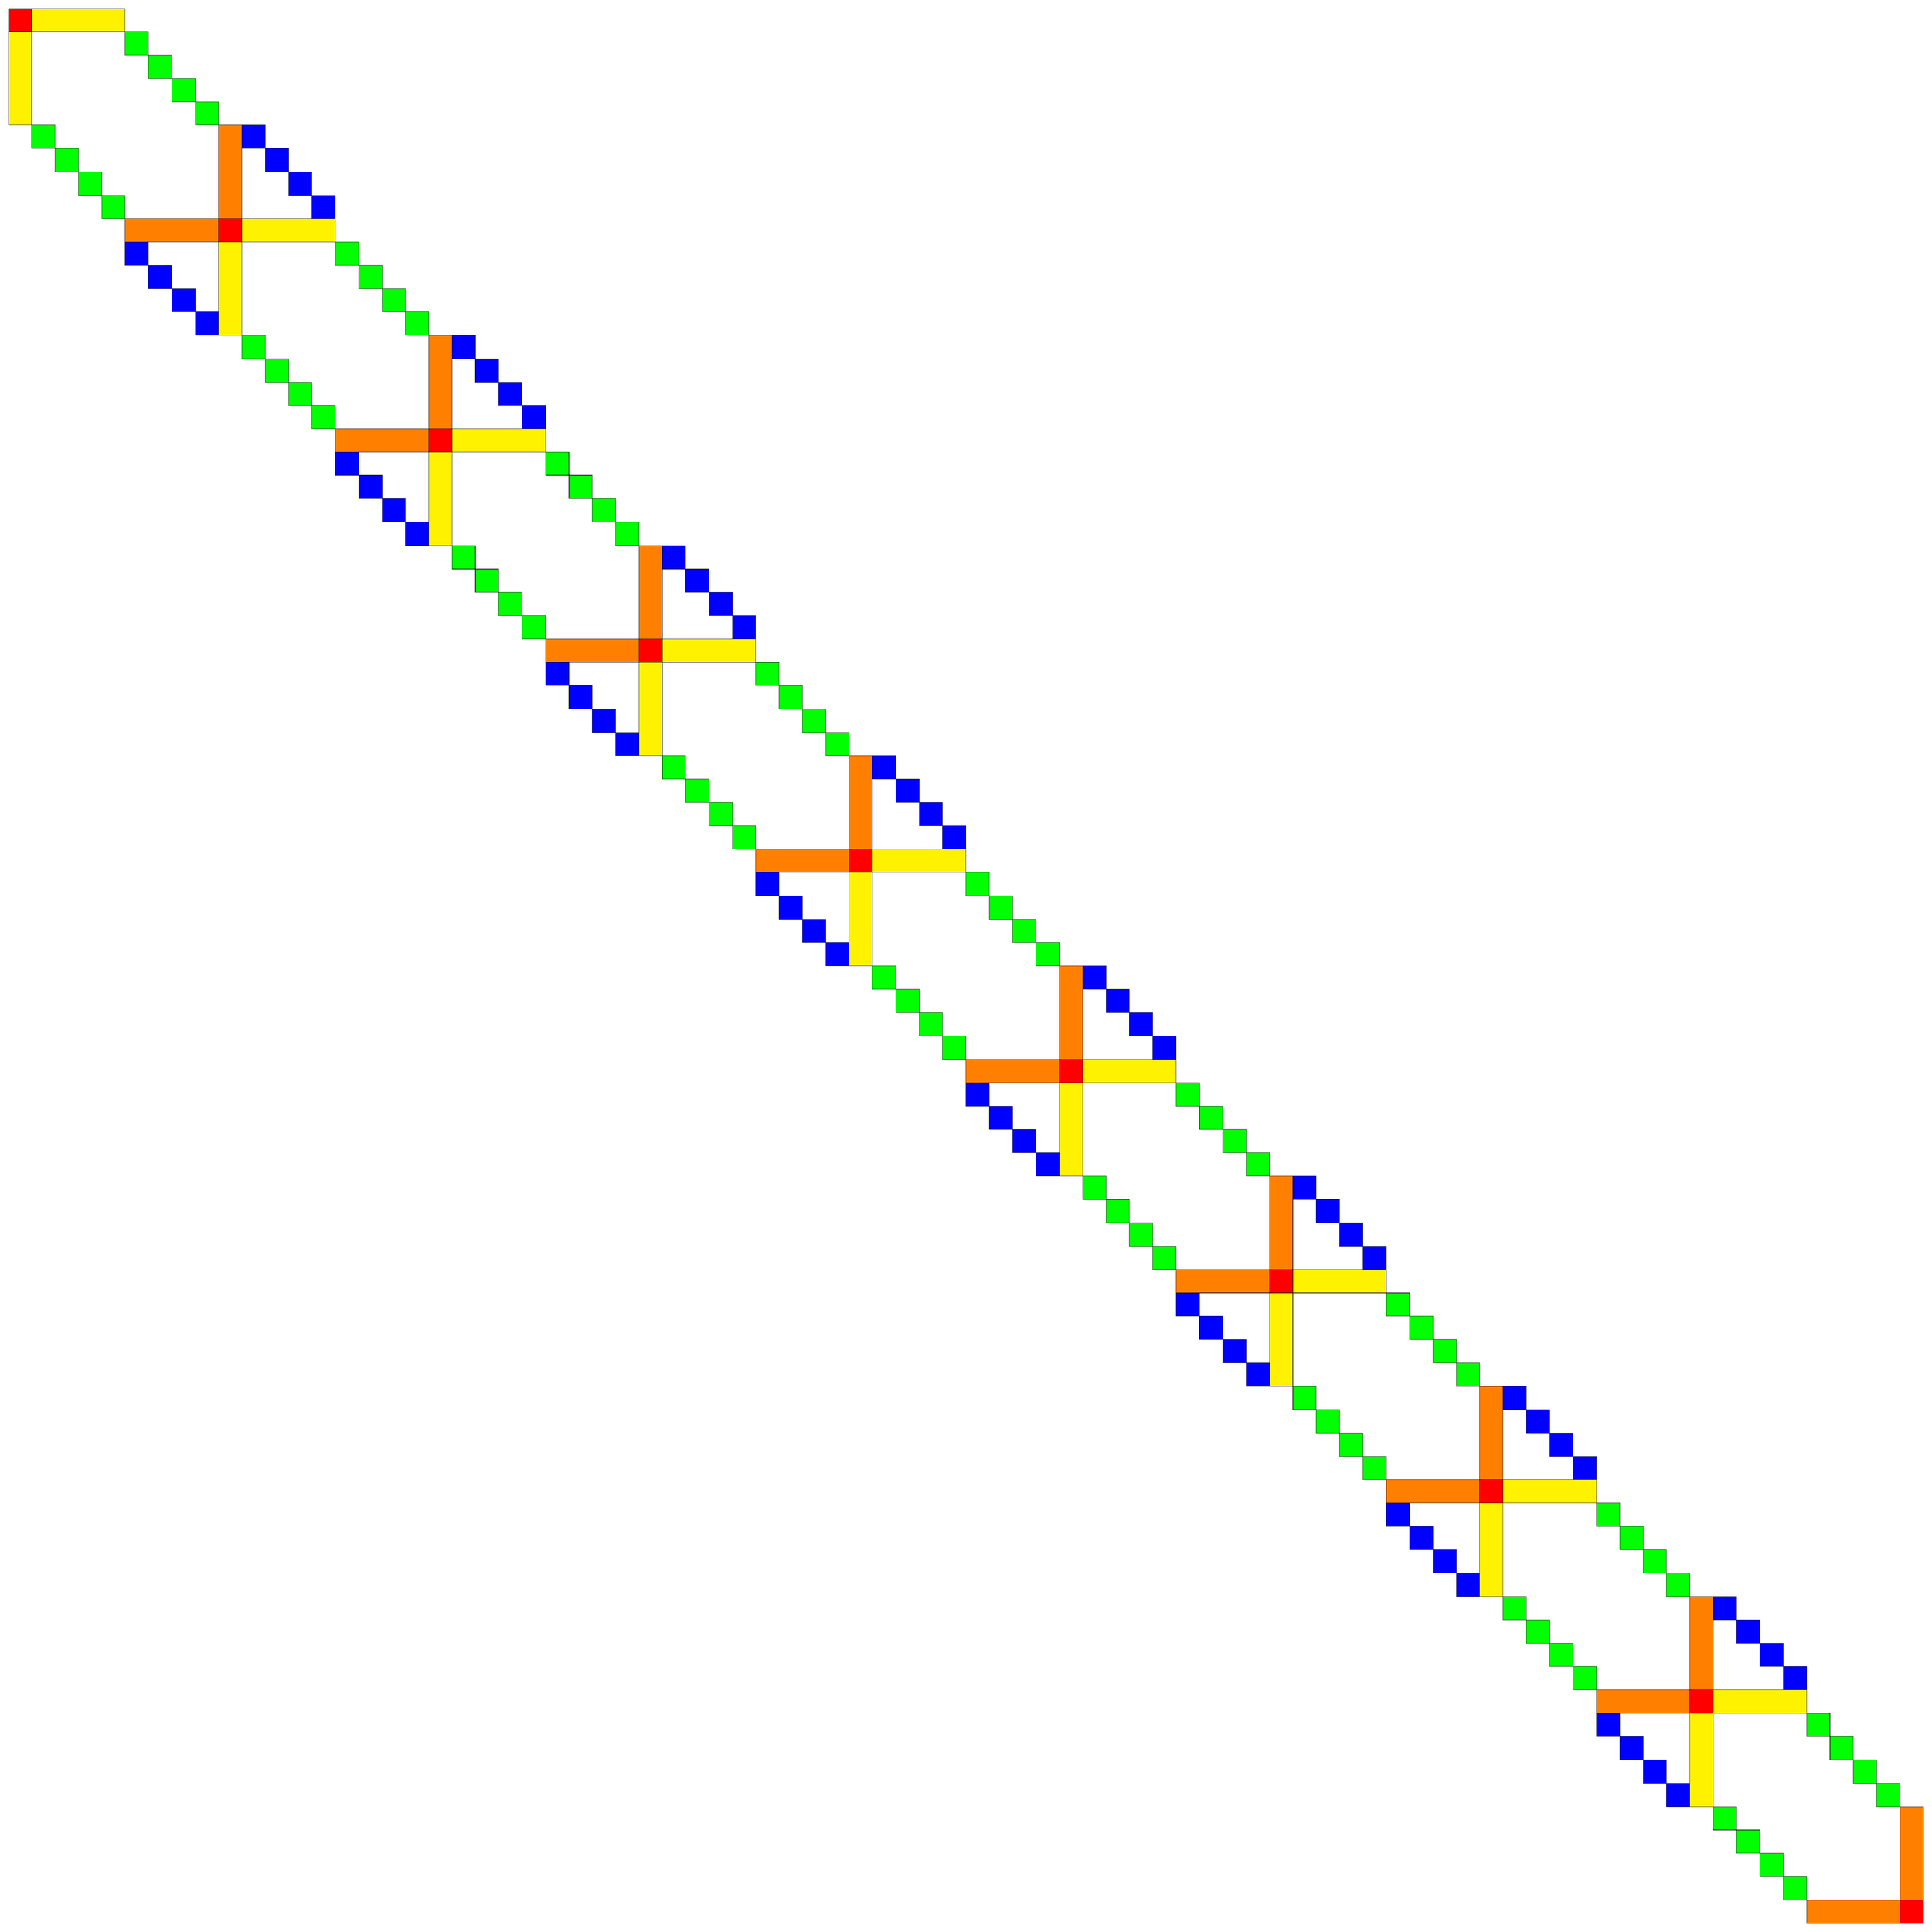
\begin{tikzpicture}
\foreach \i in {0,...,\N} {
	\draw [fill=red](\bm*\i,-\bm*\i) rectangle (\bm*\i+1,-\bm*\i-1);
}
\foreach \i in {0,...,\NM} {
	\draw [fill=yellow](\bm*\i+1,-\bm*\i) rectangle (\bm*\i+\m+1,-\bm*\i-1);
	\draw [fill=yellow](\bm*\i,-\bm*\i-1) rectangle (\bm*\i+1,-\bm*\i-1-\m);
	\foreach \j in {1,...,\m} {
		\draw [fill=green](\bm*\i+\j+\m,-\bm*\i-\j) rectangle (\bm*\i+\j+\m+1,-\bm*\i-\j-1);
		\draw [fill=green](\bm*\i+\j,-\bm*\i-\j-\m) rectangle (\bm*\i+\j+1,-\bm*\i-\j-\m-1);
	}
	\draw [fill=orange](\bm*\i+2*\m+1,-\bm*\i-\m-1) rectangle (\bm*\i+2*\m+2,-\bm*\i-\bm);
	\draw [fill=orange](\bm*\i+\m+1,-\bm*\i-\bm) rectangle (\bm*\i+\bm,-\bm*\i-\bm-1);
}
\foreach \i in {0,...,\NMM} {
	\foreach \j in {1,...,\m} {
		\draw [fill=blue](\bm*\i+2*\m+1+\j,-\bm*\i-\m-\j) rectangle (\bm*\i+2*\m+2+\j,-\bm*\i-\m-1-\j);
		\draw [fill=blue](\bm*\i+\m+\j,-\bm*\i-2*\m-1-\j) rectangle (\bm*\i+\m+1+\j,-\bm*\i-2*\m-2-\j);
	}
}
\end{tikzpicture}
\end{document}